\section{Two colour LED module}
\begin{figure}[H]
    \centering
    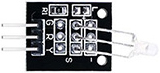
\includegraphics[angle=0, keepaspectratio=true, scale=1, width=200px, height=200px]{images/2_led.jpg}
    %\caption{Caption}
\end{figure}
\subsection*{Description}
This module functions in exactly the same way a regular three colour RGB module, simply with the omission of the blue colour pin. The LED module can be controlled by both digital and analog input signals.
\subsection*{Pin mapping}
This pin mapping corresponds to the pins from left to right with the module pins facing towards you.
\begin{table}[H]
    \centering
    \begin{tabular}{|c|c|c|c|c|}
    \hline
    Index &Label &Type &Name &Description\\ \hline
    0 &- &Ground &GND &\\ \hline
    1 & &Analog input  &A0 &Analog input signal for green pin \\ \hline
    2 &S &Analog input  &A1 &Analog input signal for red pin \\ \hline
    \end{tabular}
    %\caption{Caption}
    %\label{tab:my_label}
\end{table}
\subsection*{Operation}
By applying a PWM signal with varying duty cycle to any of the two pins (A0 and A1) we can control the brightness of each of the two primary colours. Turning both colours on at the same time "adds" them together to create other colours.
\subsection*{Code}
Refer to listing \ref{python_twocoloredled}.
%\lstinputlisting[caption=test]{laser.py}